\chapter{Introducción}

La proyección de imágenes sobre una superficie plana mediante un foco luminoso es una técnica con variadas aplicaciones, siendo de las más utilizadas la proyección de películas cinematográficas. En los últimos tiempos se introdujeron dispositivos de video que permiten proyectar la salida de una computadora, los cuales son comúnmente utilizados en ámbitos académicos y empresariales con fines de dictado de cursos y presentaciones.

En los últimos años se ha ido popularizando la proyección de imágenes y videos sobre fachadas, monumentos u otros tipos de superficies irregulares de modo de resaltar, ocultar o transformar distintas regiones de interés. Esta técnica recibe el nombre de \emph{video mapping}. Un espectáculo de \emph{video mapping} es, en esencia, una expresión artística en la que un \emph{VJ}$^\dagger$\footnote{El símbolo (\dag) representa las referencias al glosario.} presenta su creación mediante la proyección de diversos efectos visuales que generalmente son acompañados por efectos de sonido. Todo esto se logra mediante la utilización de software especializado que distorsiona las imágenes y videos proyectados.

Esta técnica tiene una gran variedad de aplicaciones que van desde el ámbito artístico hasta el publicitario. 
Es muy común observar este tipo de proyecciones sobre fachadas con la finalidad de celebrar el aniversario de algún edificio emblemático o durante la realización de festivales que se llevan a cabo periódicamente en ciertas ciudades. Claro ejemplo de esto último es el Festival de Lyon \cite{FestivalLyon} que se lleva a cabo en dicha ciudad, generando una atracción de interés turístico.
Otro tipo de aplicación de \emph{video mapping} se da en espectáculos de menor envergadura, realizados generalmente en espacios cerrados, los cuales se basan en proyecciones sobre objetos tridimensionales. Estos pueden ser tanto objetos creados específicamene para este propósito, por ejemplo maquetas, u objetos ya existenes de la más diversa variedad: automóviles, teléfonos móviles, calzado, etc. Una nueva tendencia en el ambiente artístico es la incorporación de esta técnica en obras teatrales, lográndose una ilusión de interacción entre los actores y las imágenes proyectadas.\footnote{En el presente documento todas las imágenes se referencian en el índice de figuras.}

\begin{figure}[H]
  \centering
    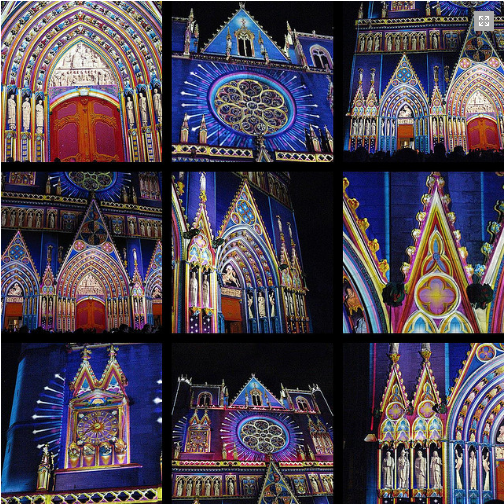
\includegraphics[width=0.6\textwidth]{./Cap1_intro/Fachada1.png}
  \caption[http://www.weltlighting.com/]{Fachada festival Lyon}
  \label{fig:Fachada1}
\end{figure}

\begin{figure}[H]
  \centering
    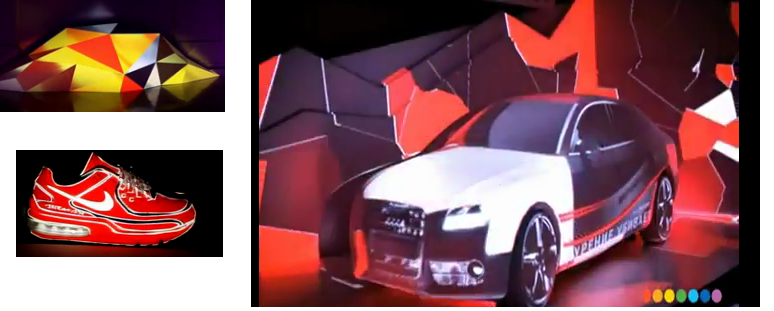
\includegraphics[width=0.75\textwidth]{./Cap1_intro/instalacion3.png}
	\caption[http://media.radugadesign.com,http://blog.naver.com/eyetive,http://www.weltlighting.com/fragment]{Instalaciones sobre maquetas.}
  \label{fig:Instalacion}
\end{figure}

\begin{figure}[H]
  \centering
    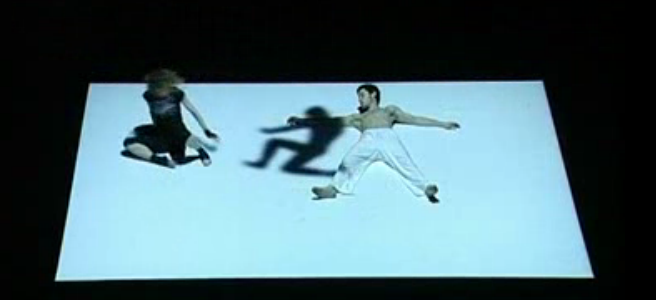
\includegraphics[width=0.75\textwidth]{./Cap1_intro/instalacionHumano1.png}
  \caption[http://www.mndl.hu/nos]{Instalación interactiva con actores.}
  \label{fig:Interactiva}
\end{figure}

Para la elaboración de un espectáculo con las características antedichas no existe un procedimiento estándar a seguir sino que cada artista utiliza sus técnicas, métodos y aplicaciones de software que considere adecuadas. No obstante, se identifican etapas comunes como la construcción de un modelo de la escena, la producción del espectáculo y su proyección. A su vez se identifican dificultades comunes como la generación del modelo y la calibración de los proyectores al momento de la reproducción.

En los siguientes capítulos, se estudian distintos métodos para facilitar la obtención del modelo virtual. En particular se relevan métodos de escaneo y reconstrucción de objetos tridimensionales y se implementa una de las estrategias estudiadas para su generación.
Se desarrolla también una aplicación que permite la creación, edición y reproducción de un espectáculo de \emph{video mapping} basada en un motor tridimensional$^\dagger$. Ésta combina la edición y la reproducción permitiendo visualizar en tiempo real los distintos efectos diseñados. A su vez permite distribuir la reproducción entre varias computadoras, asociadas a uno o más proyectores, sincronizadas todas por un componente central.

El presente documento se organiza en cuatro capítulos y cuatro apéndices, cuya temática se detalla a continuación:
\begin{itemize}
\item Capítulo 1 - Introducción a la técnica de \emph{video mapping}.
\item Capítulo 2 - Estado del arte. Explicación de las nociones básicas de la técnica y de las etapas en el proceso de creación: modelado, producción y proyección; presentación de estas dos etapas mediante los enfoques bidimensional y tridimensional; explicación de distintos algoritmos y técnicas para la obtención automática y la reconstrucción de geometría tridimensional.
\item Capítulo 3 - Solución planteada. Presentación de la solución propuesta: una herramienta para la edición y posterior ejecución de espectáculos de \emph{video mapping}.
\item Capítulo 4 - Conclusiones y trabajo futuro. Resumen de las conclusiones y posibles líneas de trabajo futuro.
\item Apéndice A - Relevamiento de aplicaciones de \emph{video mapping}. Presentación de un relevamiento de las aplicaciones existentes más populares, utilizadas para la creación de espectáculos.
\item Apéndice B - Aportes. Presentación de los resultados de una serie de entrevistas realizadas a \emph{VJs} e ingenieros que contribuyeron a la investigación del estado del arte.
\item Apéndice C - Método de triangulación. Detalle del método de triangulación utilizado para la obtención automática de geometría tridimensional.
\item Apéndice D - Modelo de cámara. Explicación de los fundamentos teóricos del modelo de cámara.
\end{itemize}